\section{Scale dependent systematics}\label{sec:scalesys}
We investigate the dependence of statistical significance for the cross power spectrum $\chi^{2}$ between the DR9 LRG targets and imaging maps. We extend the highest harmonic mode from $\ell=20$ to $100$, which corresponds to density fluctuations on scales below $2$ degrees. As shown in Figure \ref{fig:chi2cellextend}, the solid line represents the median of the cross power spectrum $\chi^{2}$ measured from the $\fnl=0$ mocks as a function of highest mode, $\ell_{\rm max}$ increases from $20$ to $100$. The red circles and blue crosses show the chi2 values for our sample cleaned respectively with the linear and neural network approaches, both with \textit{three maps}.  This test supports that our cross spectrum $\chi^{2}$ values are stable. 

\begin{figure}
\centering
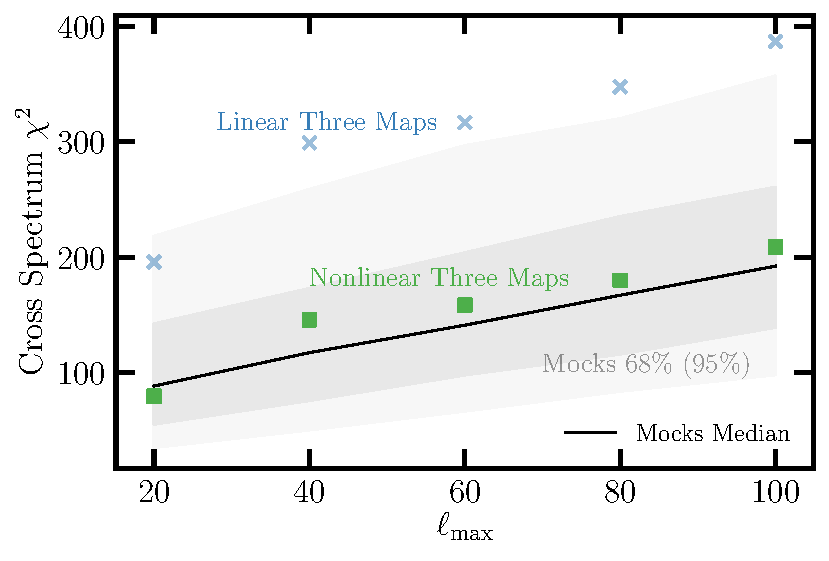
\includegraphics[width=0.45\textwidth]{chi2lmax.pdf}
\caption{The cross power spectrum $\chi^{2}$ between the DESI targets and imaging maps as a function of the highest mode $\ell_{\rm max}$ for the linear and nonlinear three maps imaging weights. The lowest mode is fixed at $\ell_{\rm min}=2$. Solid curve and dark (light) shade represent the median estimate and $68\%$ ($95\%$) confidence regions from the $\fnl=0$ mocks.}\label{fig:chi2cellextend}
\end{figure}


\section{Uncalibrated constraints from DR9}\label{sec:dr9uncalib}

\begin{figure}
    \centering
    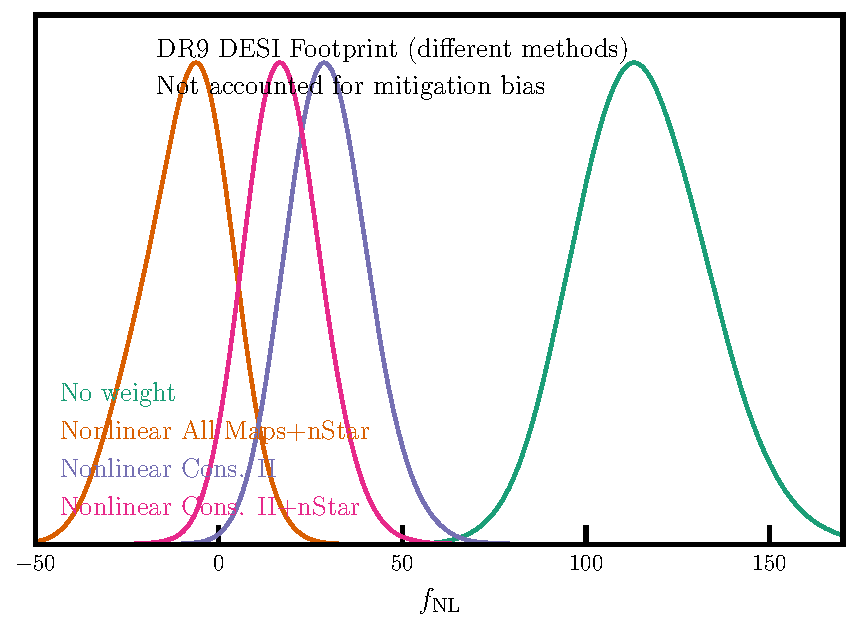
\includegraphics[width=0.45\textwidth]{figures/mcmc_dr9methods1dnoshift.pdf}
    \caption{Probability distribution of $\fnl$ from the DR9 LRG targets. The distributions are not debiased for over-correction.}
    \label{fig:mcmcdr9noshift}
\end{figure}


\section{Lognormal mocks}
Corner plots of the PNG parameter $\fnl$ and bias coefficient are shown in Fig. \ref{fig:mcmc_mocks0} for fitting the mean power spectrum of mocks, with and without $\fnl$. Best fit estimates, marginalized mean, $1\sigma$ and $2\sigma$ confidence intervals are summarized in Tab. \ref{tab:mocksmcmc}. Fig \ref{fig:mcmc_mocks0} (right) shows confidence contours for different combinations of target variable (e.g., either power spectrum or its log transform) and covariance matrix. First we attempt to understand the impact of covariance on confidence intervals. We fit the mean power spectrum of $\fnl=76.9$ mocks or its log transformation using covariance matrices constructed from the same set of mocks or from the $\fnl=0$ mocks. When covariance is consistent with mean, the difference between fitting power spectrum and log of it is only 2\%. If a wrong covariance is used for the log power, the effect is only $7\%$. However, when mean power spectrum of the $\fnl=76.9$ mocks is fit using the covariance matrix estimated from the $\fnl=0$ mocks, the constraints improve by a factor of $5$, simply due to a false higher signal to noise ratio. Therefore, we argue that fitting logarithm of power spectrum would remove the need for having $\fnl$-dependent covariance matrices and make the constraints less sensitive to covariance construction. Fig. \ref{fig:mcmc_mocks0} shows the confidence contours for $\fnl=0$ mocks when fit is done to the log of mean spectra of $\fnl=0$ mocks for the different regions. We find that the underlying true $\fnl$ value is recovered within $2\sigma$ confidence. \mr{Add a paragraph for the constraining power vs fsky}.

Fig \ref{fig:bestfit_mocks} shows the best fit estimates for $b$ vs $\fnl$ for $\fnl=0$ and $=76.92$ mocks in the left and right, respectively. Truth values are represented via the dotted lines. The points are color-coded with the minimum $\chi^{2}$ from fit for each realization. The histograms of best fit $\fnl$ estimates are plotted in the background.

\begin{table*}
  %\begin{center}
    \caption{Best fit and marginalized mean estimates for $\fnl$ from fitting the mean power spectrum of the mocks. Degree of freedom is 34 (37 data points - 3 parameters).}   
    \label{tab:mocksmcmc}  
   \centerline{%
    \begin{tabular}{llllllll}
    \hline
    \hline
   &  & & & & $\fnl$ &  \\
   \cmidrule(r{.7cm}){4-7}    
Mock / $\fnl$ &  Footprint   &  Observable & 	Best fit  & Mean & $ 68\%$ CL & $ 95\%$ CL & $\chi^{2}$ \\
    \hline
Clean $76.92$ & DESI & log$C_{\ell}$    & $ 77.67$& $ 77.67$& $ 77.17<\fnl< 78.16$& $ 76.71<\fnl< 78.64$ &   38.8\\
Clean $76.92$ & DESI & $C_{\ell}$       & $ 77.67$& $ 77.65$& $ 77.17<\fnl< 78.14$& $ 76.70<\fnl< 78.60$ &   39.0\\
Clean $76.92$ & DESI & log$C_{\ell}$ + $f_{\rm NL}=0$ cov & $ 77.70$& $ 77.71$& $ 77.25<\fnl< 78.17$& $ 76.81<\fnl< 78.63$ &   39.9\\
Clean $76.92$ & DESI & $C_{\ell}$ + $f_{\rm NL}=0$ cov & $ 77.03$& $ 77.02$& $ 76.93<\fnl< 77.12$& $ 76.83<\fnl< 77.22$ &  207.6\\
\hline
Clean $0$ & DESI         &  log$C_{\ell}$ & $  0.36$& $  0.36$& $  0.06<\fnl<  0.65$& $ -0.23<\fnl<  0.94$ &   35.7\\
Clean $0$ & BASS+MzLS    &  log$C_{\ell}$ & $  0.83$& $  0.82$& $  0.25<\fnl<  1.40$& $ -0.31<\fnl<  1.96$ &   39.4\\
Clean $0$ & DECaLS North &  log$C_{\ell}$& $  0.07$& $  0.06$& $ -0.47<\fnl<  0.60$& $ -1.00<\fnl<  1.12$ &   26.7\\
Clean $0$ & DECaLS South &  log$C_{\ell}$& $  0.67$& $  0.67$& $  0.13<\fnl<  1.22$& $ -0.40<\fnl<  1.75$ &   34.3\\
\hline
    \end{tabular}
    }
\end{table*}


\begin{figure}
    \centering
    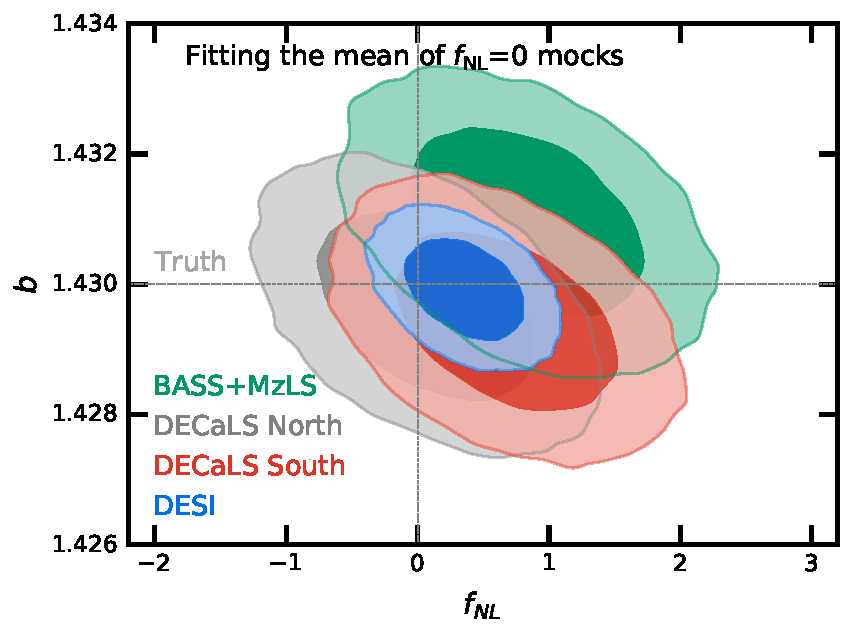
\includegraphics[width=0.45\textwidth]{figures/mcmc_zero.pdf} 
    \caption{68\% and 95\% confidence contours from the mean power spectrum of the $\fnl=0$ mocks for the DESI footprint and sub-imaging surveys. The truth values are represented by vertical and horizontal lines.}\label{fig:mcmc_mocks0}
\end{figure}

\begin{figure}
    \centering
    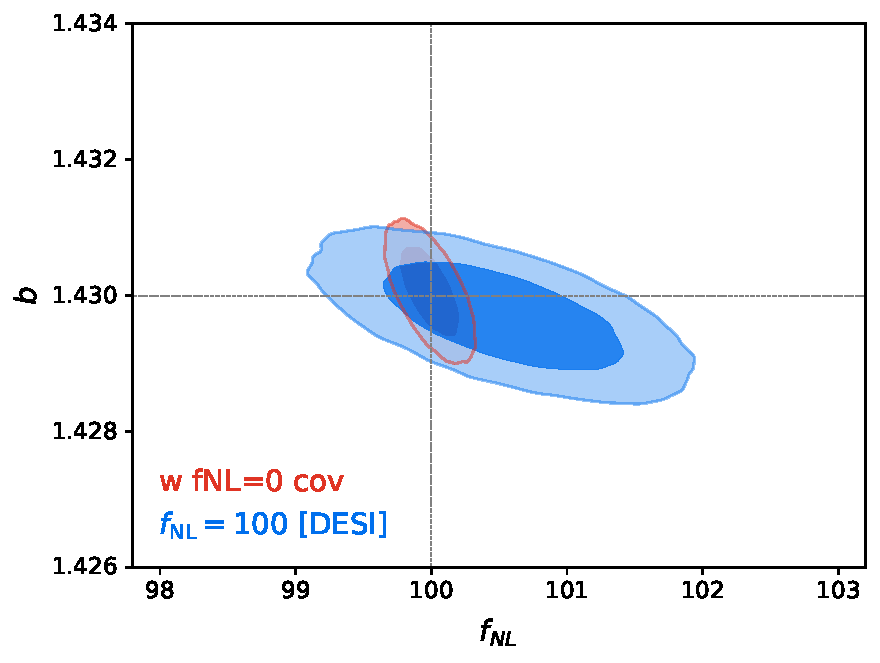
\includegraphics[width=0.45\textwidth]{figures/mcmc_po100.pdf} 
    \caption{68\% and 95\% confidence contours of fitting the mean power spectrum or its log transformation from the $\fnl=76.92$ mocks for the DESI footprint. Using the $\log C_{\ell}$ fitting yield constraints that are insensitive to the covariance used. The truth values are represented by vertical and horizontal lines.}\label{fig:mcmc_mocks100}
\end{figure}

\begin{figure}
    \centering
    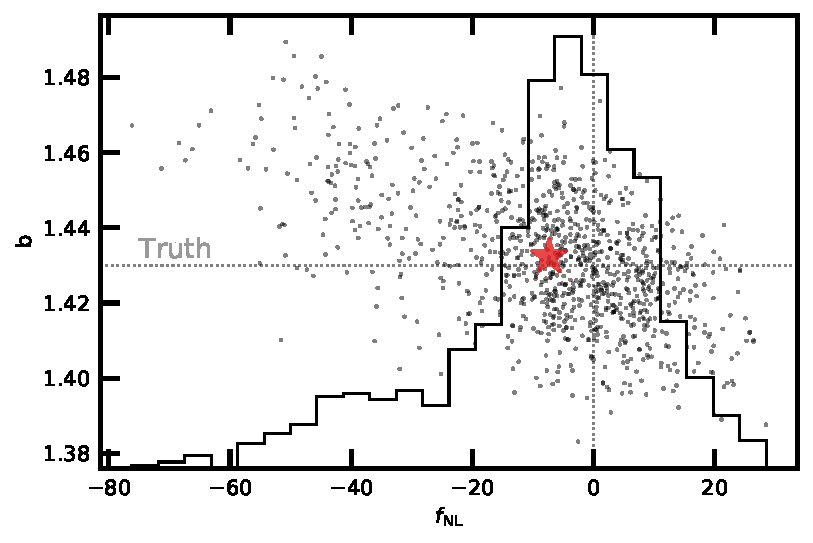
\includegraphics[width=0.45\textwidth]{figures/bestfit_zero.pdf} 
    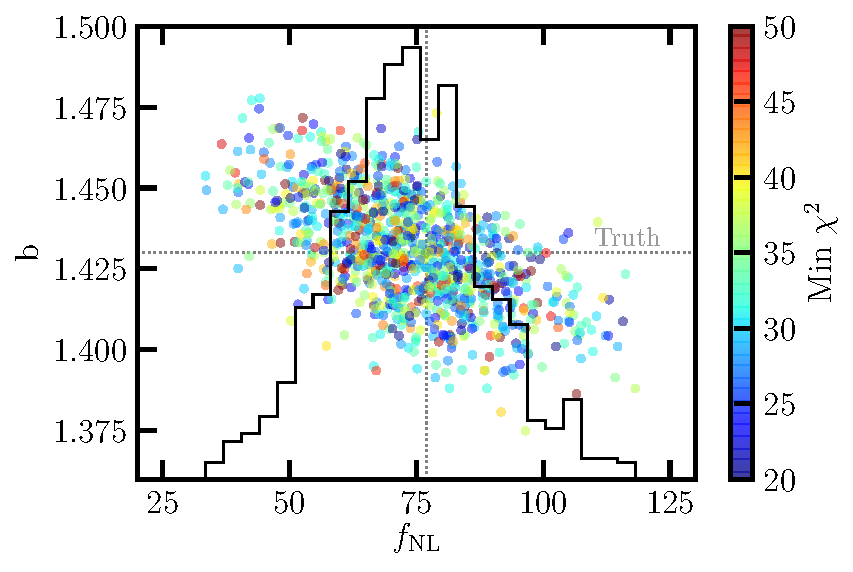
\includegraphics[width=0.45\textwidth]{figures/bestfit_po100.pdf}         
    \caption{Top: 68\% and 95\% confidence contours for $\fnl=0$ (left) and $76.92$ (right) mocks. Using the $\log C_{\ell}$ fitting yield constraints that are insensitive to the covariance used. Bottom: best fit estimates from fitting 1000 lognormal mocks with $\fnl=0$ (left) and $76.92$ (right) in the DESI footprint. The truth values are represented by vertical and horizontal lines.\textcolor{olive}{up and down figures?}}\label{fig:bestfit_mocks}
\end{figure}




% \subsubsection{Contaminated density fields}\label{ssec:contmocks}

\begin{table*}
  %\begin{center}
    \caption{Best fit and marginalized estimates for $\fnl$ from fitting the mean power spectrum of the mocks before and after applying imaging weights. }   
    \label{tab:contmocksmcmc}  
   \centerline{%
    \begin{tabular}{lllllll}
    \hline
    \hline
   &  & 	  & & & $\fnl$ &  \\
   \cmidrule(r{.7cm}){3-6}    
Mock / $\fnl$ & Method & Best fit  & Mean & $ 68\%$ CL & $ 95\%$ CL & $\chi^{2}$ \\
    \hline
Clean $0$ & No Weight                   & $  0.36$& $  0.36$& $  0.06<\fnl<  0.65$& $ -0.23<\fnl<  0.94$ &   35.7\\
Clean $0$ & Three Maps                  & $-11.64$& $-11.65$& $-12.00<\fnl<-11.30$& $-12.34<\fnl<-10.97$ &   86.8\\
Clean $0$ & Four Maps                   & $-20.14$& $-20.13$& $-20.44<\fnl<-19.82$& $-20.74<\fnl<-19.52$ &  472.8\\
Clean $0$ & Nine Maps                   & $-26.91$& $-26.92$& $-27.16<\fnl<-26.68$& $-27.39<\fnl<-26.46$ & 5481.0\\
Contaminated $0$ & Three Maps           & $-12.12$& $-12.13$& $-12.48<\fnl<-11.78$& $-12.83<\fnl<-11.44$ &   94.0\\
Contaminated $0$ & Four Maps            & $-20.97$& $-20.98$& $-21.28<\fnl<-20.67$& $-21.58<\fnl<-20.37$ &  556.3\\
Contaminated $0$ & Nine Maps            & $-28.13$& $-28.13$& $-28.36<\fnl<-27.90$& $-28.59<\fnl<-27.67$ & 6760.5\\
Clean $76.92$ & No Weight               & $ 77.67$& $ 77.67$& $ 77.17<\fnl< 78.16$& $ 76.71<\fnl< 78.64$ &   38.8\\
Clean $76.92$ & Three Maps              & $ 54.57$& $ 54.57$& $ 54.14<\fnl< 55.01$& $ 53.72<\fnl< 55.45$ &  603.5\\
Clean $76.92$ & Four Maps               & $ 38.38$& $ 38.38$& $ 37.99<\fnl< 38.78$& $ 37.60<\fnl< 39.16$ &  537.0\\
Clean $76.92$ & Nine Maps               & $  6.04$& $  6.04$& $  5.72<\fnl<  6.36$& $  5.41<\fnl<  6.67$ &  694.0\\
Contaminated $76.92$ & Three Maps       & $ 54.01$& $ 54.00$& $ 53.57<\fnl< 54.44$& $ 53.15<\fnl< 54.86$ &  588.0\\
Contaminated $76.92$ & Four Maps        & $ 37.48$& $ 37.49$& $ 37.09<\fnl< 37.88$& $ 36.70<\fnl< 38.27$ &  510.7\\
Contaminated $76.92$ & Nine Maps        & $  4.59$& $  4.58$& $  4.26<\fnl<  4.90$& $  3.95<\fnl<  5.22$ &  649.7\\
\hline
    \end{tabular}
    }
\end{table*}


\begin{figure}
\centering
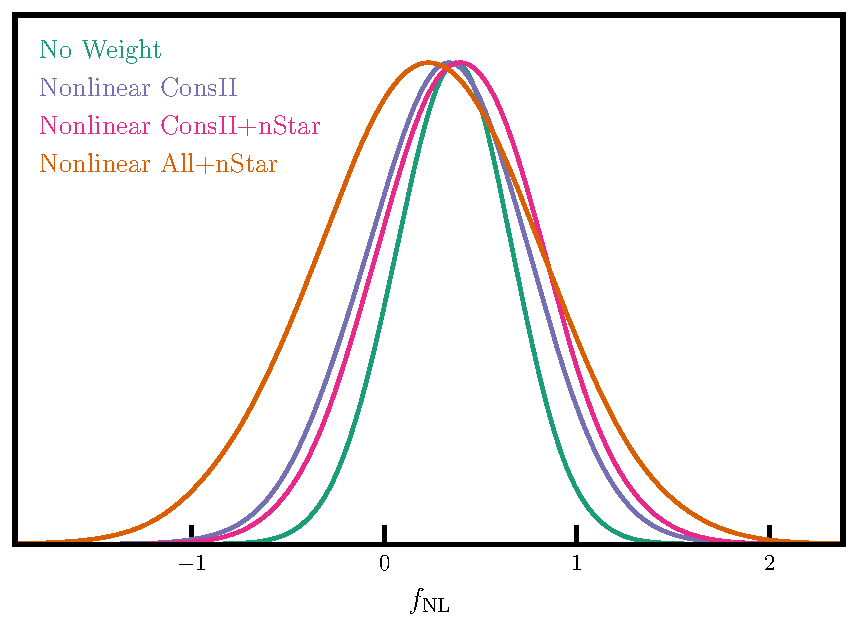
\includegraphics[width=0.45\textwidth]{figures/mcmc_cont.pdf}
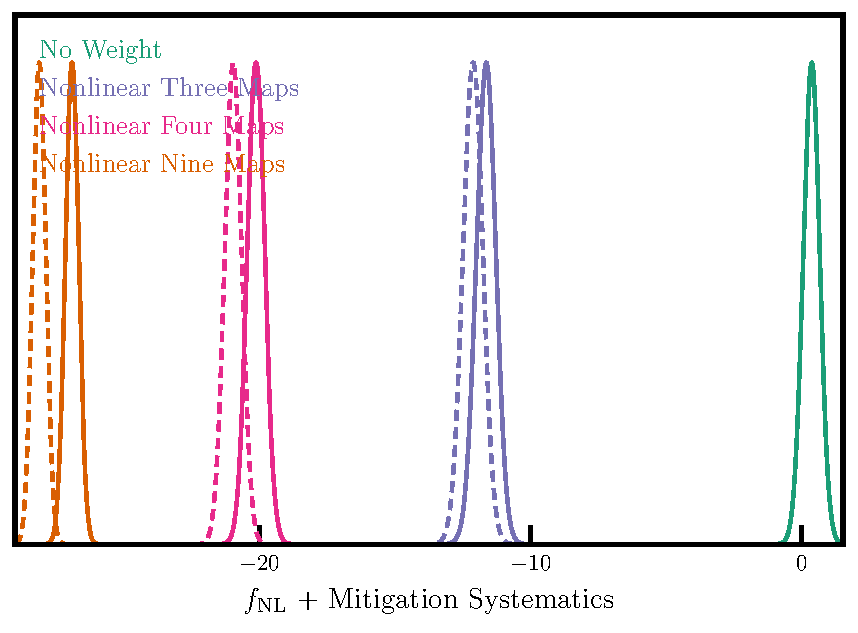
\includegraphics[width=0.45\textwidth]{figures/mcmc_contnoshift.pdf}
\caption{Probability distributions of $\fnl$ from the mean power spectrum of the $\fnl=0$ mocks before and after mitigation with nonlinear methods. Top: The mitigated posteriors are debiased for the over correction effect. Bottom: The distribtions of mitigated cases are biased because of over correction.}\label{fig:contmcmc}
\end{figure}


% \section{Redshift distribution}
% Redshift distribution of LRGs is constructed from the DESI SV data release of Denali with the same selection. The fiducial distribution only covers the redshift range from 0.2 to 1.35. Below we test the impact of LRG dN/dz on the angular power spectrum.


% \begin{figure}
% \centering
% 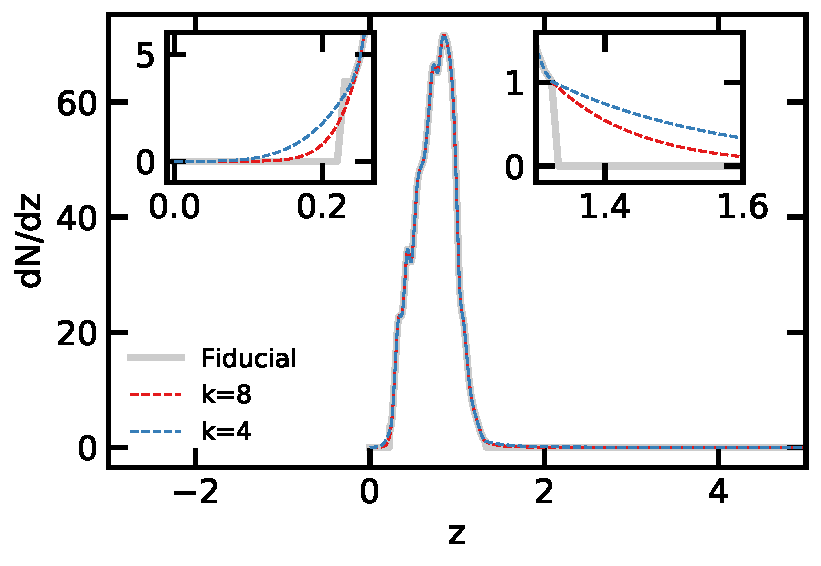
\includegraphics[width=0.45\textwidth]{nztreat.pdf}
% 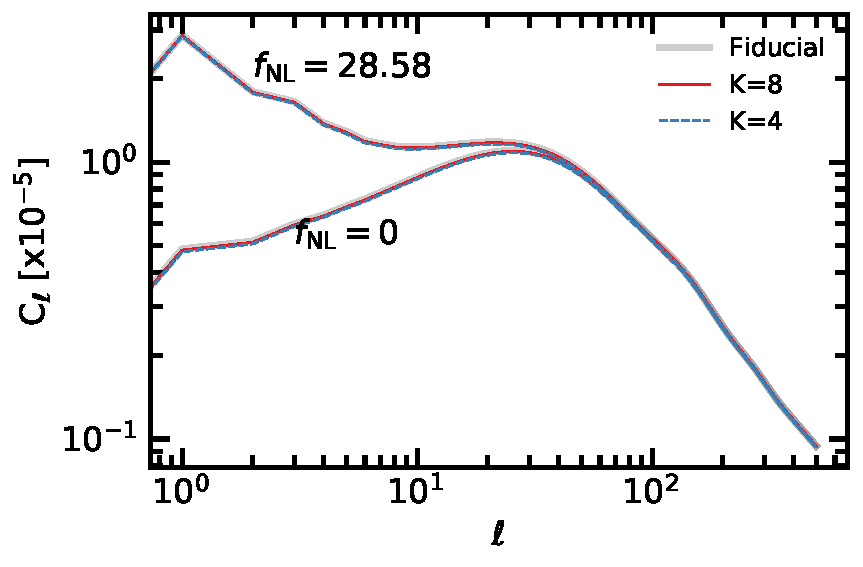
\includegraphics[width=0.45\textwidth]{cell_nz.pdf}
% \caption{Top: Redshift distribution of LRGs. Bottom: Power spectrum given various dN/dz treatments for two arbitrary $\fnl$ values.}
% \end{figure}